\begin{activity} \label{A:3.4.2}  A hiker starting at a point $P$ on a straight road walks east towards point $Q$, which is on the road and 3 kilometers from point $P$.  Two kilometers due north of point $Q$ is a cabin.  The hiker will walk down the road for a while, at a pace of 8 kilometers per hour.  At some point $Z$ between $P$ and $Q$, the hiker leaves the road and makes a straight line towards the cabin through the woods, hiking at a pace of 3 kph, as pictured in Figure~\ref{F:3.4.Act2}.  In order to minimize the time to go from $P$ to $Z$ to the cabin, where should the hiker turn into the forest?
\begin{figure}[h]
\begin{center}
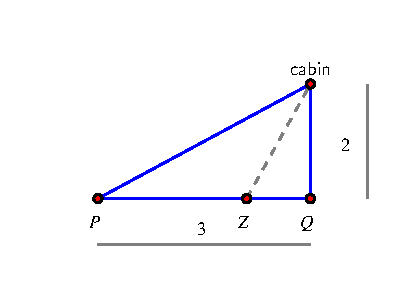
\includegraphics{figures/3_4_Act2.eps}
\caption{A hiker walks from $P$ to $Z$ to the cabin, as pictured.} \label{F:3.4.Act2}
\end{center}
\end{figure}
\end{activity}
\begin{smallhint}
Let $x$ be the distance from $Z$ to $Q$. What is then the distance from $P$ to $Z$ in terms of $x$?  How about the distance from $Z$ to the cabin?  How does time depend on distance and rate?
\end{smallhint}
\begin{bighint}
Let $x$ be the distance from $Z$ to $Q$. What is then the distance from $P$ to $Z$ in terms of $x$?  How about the distance from $Z$ to the cabin?  Remember that since distance equals rate times time, time is given by distance divided by rate.  Find an expression for the total time, $T$, as a function of $x$.
\end{bighint}
\begin{activitySolution}
We begin by letting $x$ be the distance from $Z$ to $Q$.  Since it is 3 km from $P$ to $Q$, the distance from $P$ to $Z$ is $3-x$.  Further, by the Pythagorean Theorem, the distance from $Z$ to the cabin is $\sqrt{4+x^2}$.

Next, we want to determine the hiker's time as a function of $x$.  Because distance equals rate times time, time is thus distance divided by rate.  Along the road, the hiker's distance is $3-x$ km and her rate is $8$ km/hr, thus her time on the road, $T_r$ is
$$T_r = \frac{3-x}{8}.$$
Once she enters the woods, her rate drops to $3$ km/hr and travels a distance of $\sqrt{4+x^2}$ km, making her time in the woods, $T_w$, given by
$$T_w = \frac{\sqrt{4+x^2}}{3}.$$
Thus, the hiker's total time is given by the function
$$T(x) = \frac{3-x}{8} + \frac{\sqrt{4+x^2}}{3}.$$

Because the only values of $x$ that make sense to use are $0 \le x \le 3$ (using either negative values or values greater than 3 clearly add unnecessary time to the trip), we use this domain for $T$ and now seek the absolute minimum of $T$ on $[0,3]$.  First, we find that
$$T'(x) = -\frac{1}{8} + \frac{1}{3} \cdot \frac{1}{2} (4+x^2)^{-1/2} (2x) = -\frac{1}{8} + \frac{x}{3\sqrt{4+x^2}}.$$
Setting $T'(x) = 0$ and solving for $x$, we have $\frac{x}{3\sqrt{4+x^2}} = \frac{1}{8}$, so $8x = 3\sqrt{4+x^2}$.  Squaring both sides, $64x^2 = 9(4+x^2) = 36 + 9x^2$.  Hence, $55x^2 = 36$, so $x = \sqrt{\frac{36}{55}} \approx 0.80904$.  (We don't consider the critical value $x = -\sqrt{\frac{36}{55}}$ because this doesn't lie in the relevant domain of $T$.)

Finally, we evaluate $T$ at the only critical value in the interval and at the interval's endpoints.  Doing so, we find $T(0) = \frac{3}{8} + \frac{2}{3} \approx 1.0417$, $T(3) = \frac{\sqrt{13}{3}} \approx 1.20185$, and $T(\sqrt{\frac{36}{55}}) = \frac{3}{8} + \frac{\sqrt{55}}{12} \approx 0.99302$, and thus the absolute minimum time the hiker can achieve is $0.99302$ hours, which is attained by hiking about 2.2 km from $P$ to $Q$ and then turning into the woods for the remainder of the trip.
\end{activitySolution}
\aftera